\chapter{ARIA: Field Test}
A field test was performed in a trafficked area in Padova (Italy) in autumn 2021 (see Figure \ref{fig:3d-map}), mainly to test the sensors. The drones were carried by hand. the Figures below contain the data collected by the two drones, the mission times are synchronized and the Arduino drone also has the data for the NO sensor.
Firstly, the sensors and telemetry data are synchronized, as can be verified both by comparing the UNIX times in each row of the output csv files (see Section \ref{section:software}) and by comparison of the data from the Raspberry Pi and Arduino drones in Figure \ref{fig:pms-and-sensors}. The plot, in fact, shows that the



\begin{figure}[h!]
    \centering
    \begin{subfigure}[b]{0.45\textwidth}
        \centering
        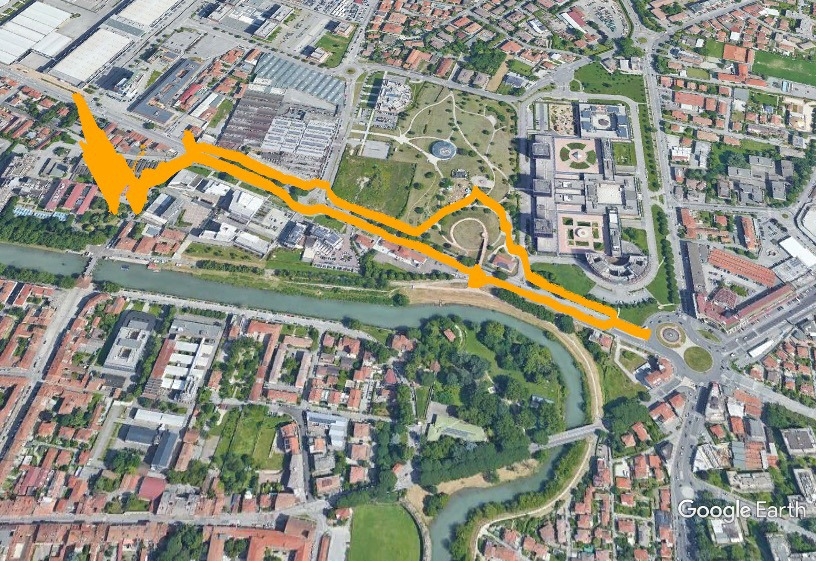
\includegraphics[width=\textwidth]{images/flight-data/3d-map.jpg}
        \caption{}
        \label{fig:3d-map}
    \end{subfigure}
    \hfill
    \begin{subfigure}[b]{0.45\textwidth}
        \centering
        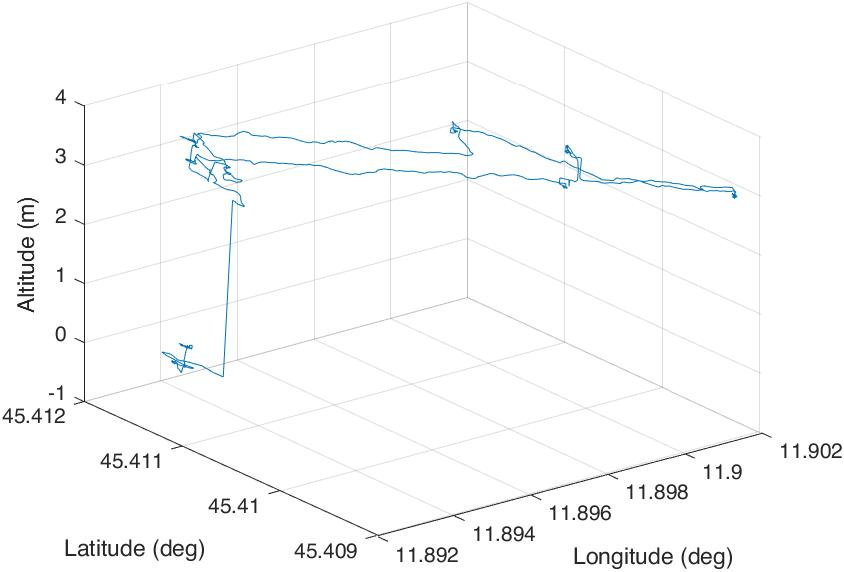
\includegraphics[width=\textwidth]{images/flight-data/raspberry/ALT_3D_R.jpg}
        \caption{}
        \label{fig:testflight-alt}
    \end{subfigure}
       \caption{3D map and 3D altitude plot}
       \label{fig:testflight-telemetry}
\end{figure}

\begin{figure}
    \centering
    \begin{subfigure}[b]{0.45\textwidth}
        \centering
        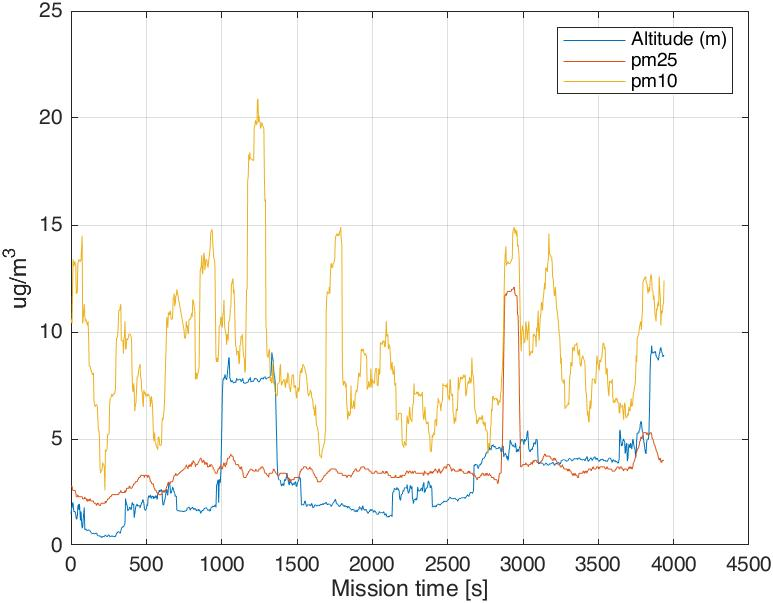
\includegraphics[width=\textwidth]{images/flight-data/raspberry/pms_R.jpg}
        \caption{Raspberry Pi drone PM sensor data}
        \label{fig:pms_R}
    \end{subfigure}
    \hfill
    \begin{subfigure}[b]{0.45\textwidth}
        \centering
        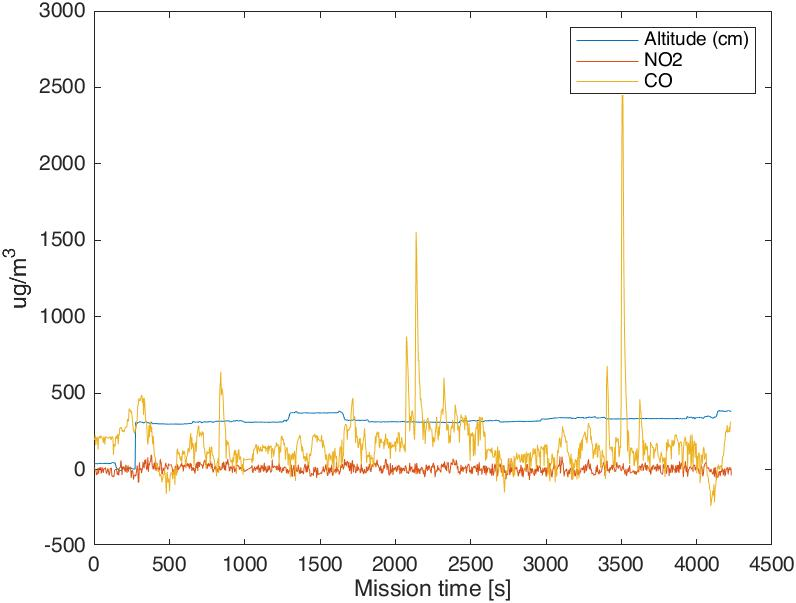
\includegraphics[width=\textwidth]{images/flight-data/raspberry/ariasensors_R.jpg}
        \caption{Raspberry Pi drone gas sensor data}
        \label{fig:ariasensors_R}
    \end{subfigure}

    \centering
    \begin{subfigure}[b]{0.45\textwidth}
        \centering
        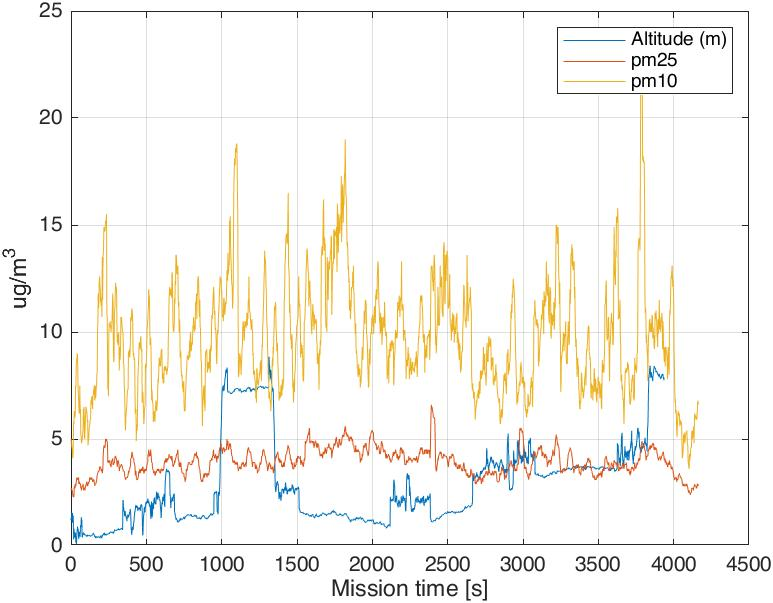
\includegraphics[width=\textwidth]{images/flight-data/arduino/pms.jpg}
        \caption{Arduino drone PM sensor data}
        \label{fig:pms}
    \end{subfigure}
    \hfill
    \begin{subfigure}[b]{0.45\textwidth}
        \centering
        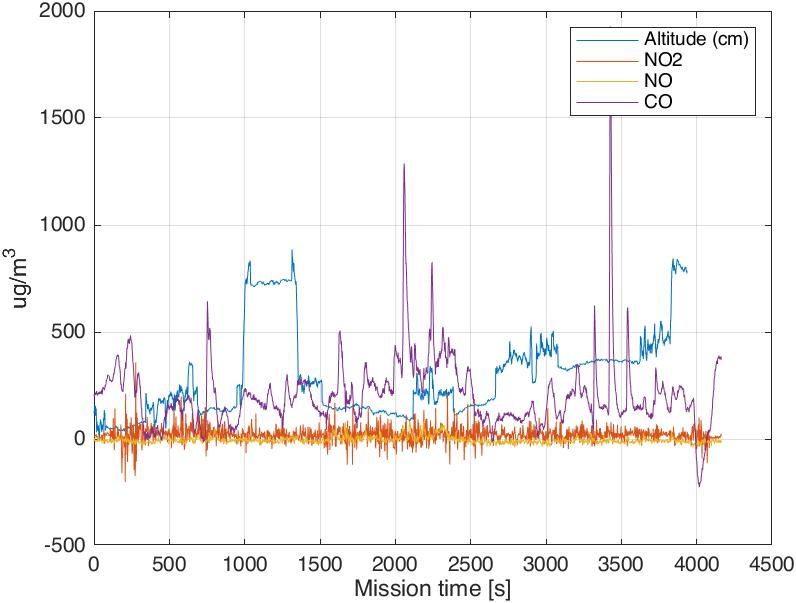
\includegraphics[width=\textwidth]{images/flight-data/arduino/ariasensors.jpg}
        \caption{Arduino drone gas sensor data}
        \label{fig:ariasensors}
    \end{subfigure}
    \hfill
       \caption{PM and gas sensors data from the Raspberry Pi drone (top two) and the Arduino drone (bottom two)}
       \label{fig:pms-and-sensors}
\end{figure}

\begin{figure}
    \centering
    \begin{subfigure}[b]{0.45\textwidth}
        \centering
        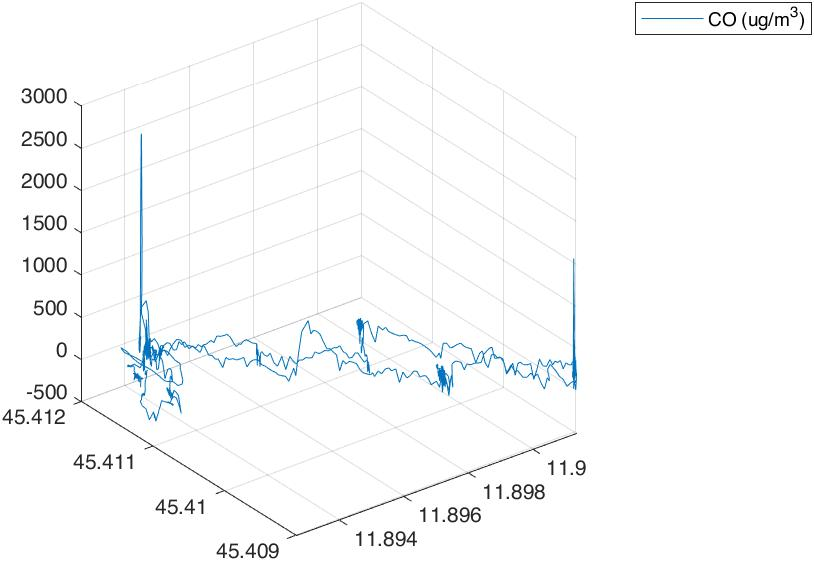
\includegraphics[width=\textwidth]{images/flight-data/raspberry/CO_3D_R.jpg}
        \caption{Raspberry Pi $CO$}
        \label{fig:CO_3D_R}
    \end{subfigure}
    \hfill
    \begin{subfigure}[b]{0.45\textwidth}
        \centering
        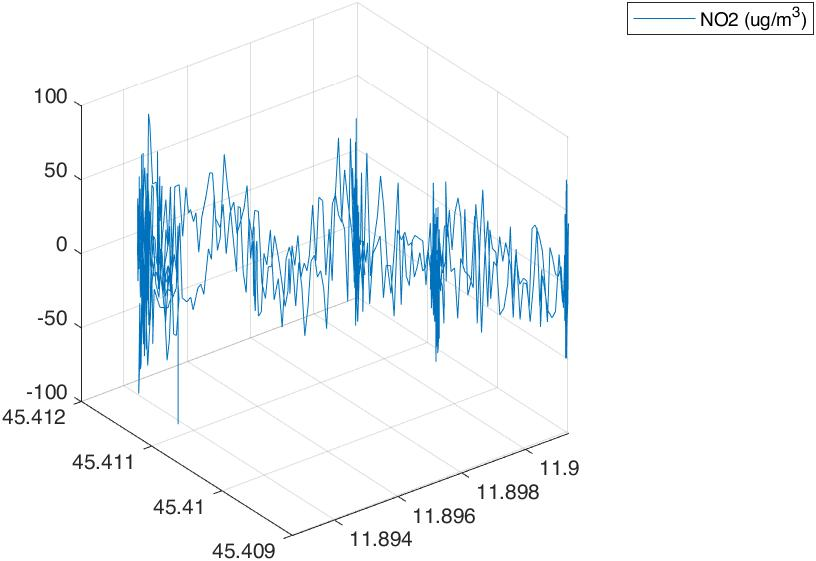
\includegraphics[width=\textwidth]{images/flight-data/raspberry/NO2_3D_R.jpg}
        \caption{Raspberry Pi $NO_2$}
        \label{fig:NO2_3D_R}
    \end{subfigure}

    \centering
    \begin{subfigure}[b]{0.45\textwidth}
        \centering
        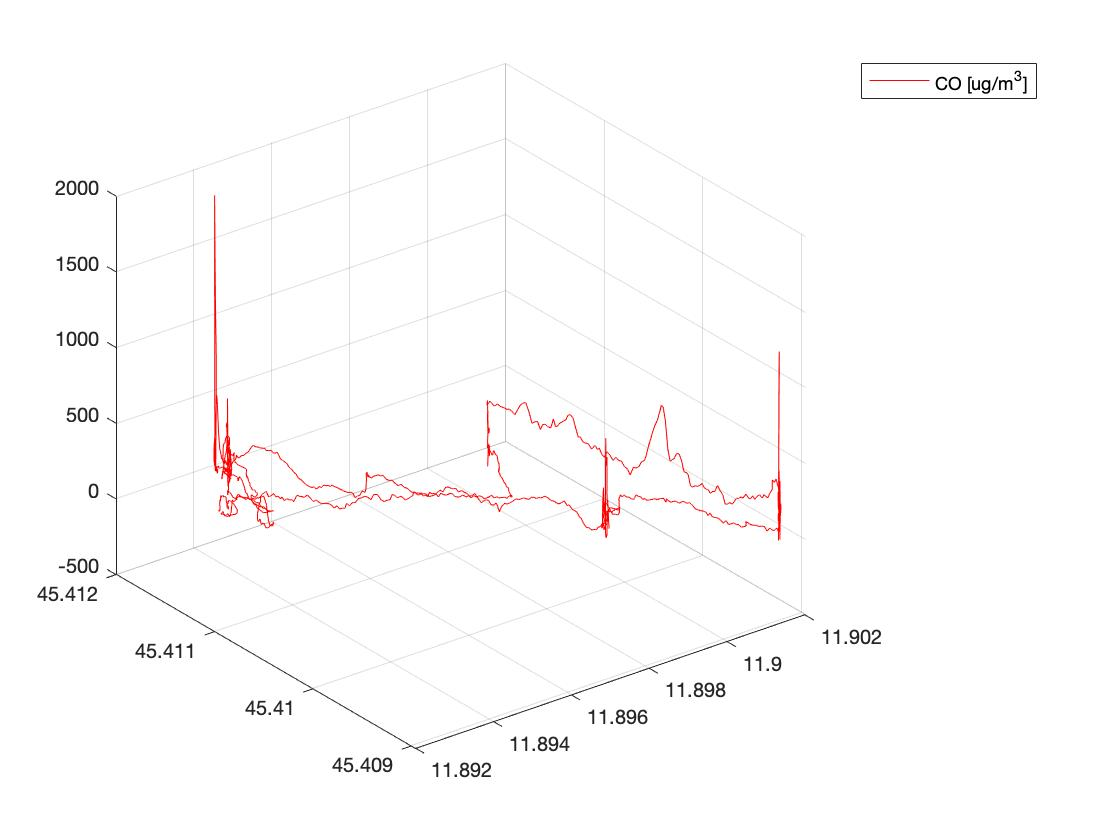
\includegraphics[width=\textwidth]{images/flight-data/arduino/CO_3D.jpg}
        \caption{Arduino $CO$}
        \label{fig:CO_3D}
    \end{subfigure}
    \hfill
    \begin{subfigure}[b]{0.45\textwidth}
        \centering
        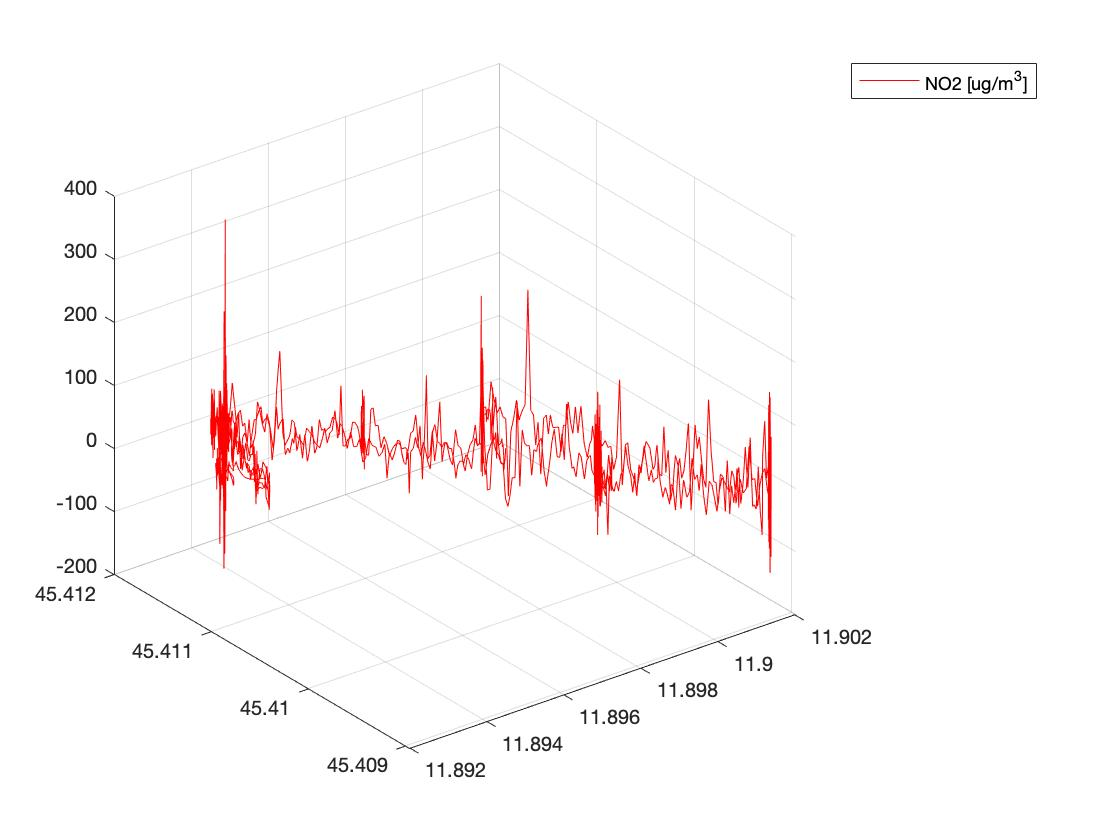
\includegraphics[width=\textwidth]{images/flight-data/arduino/NO2_3D.jpg}
        \caption{Arduino $NO_2$}
        \label{fig:NO2_3D}
    \end{subfigure}
    
    \begin{subfigure}[b]{0.45\textwidth}
        \centering
        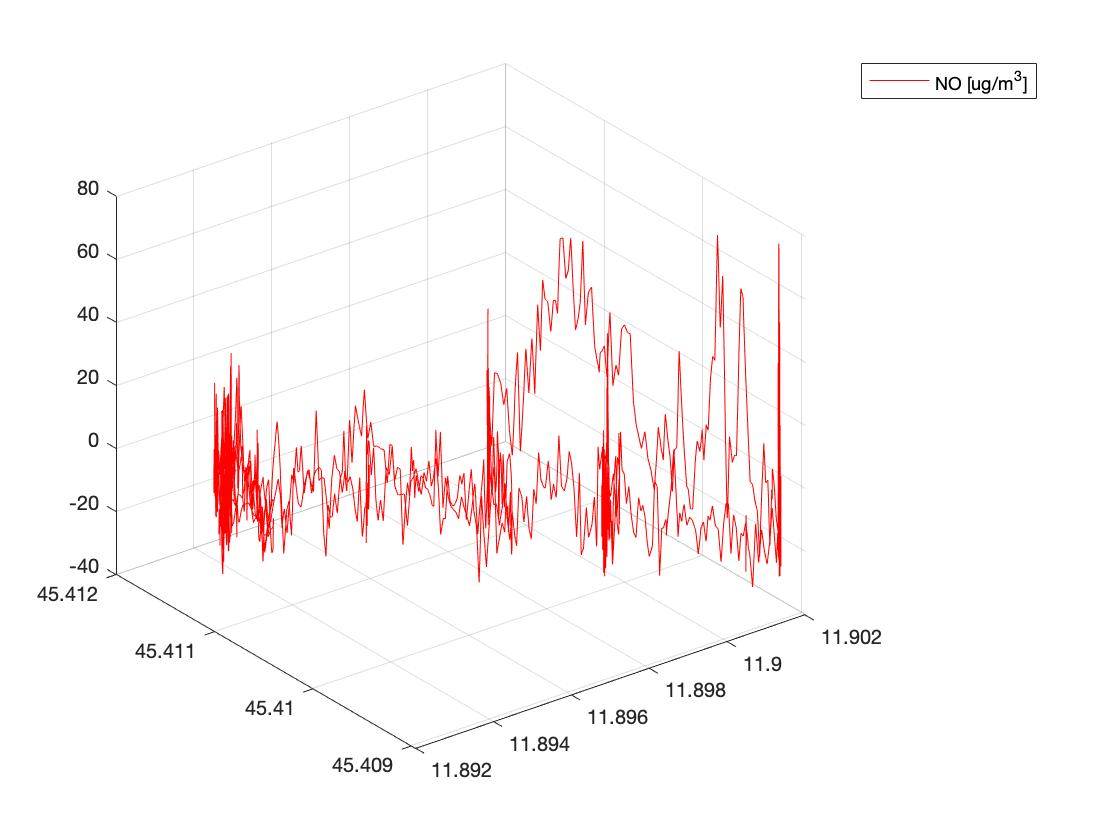
\includegraphics[width=\textwidth]{images/flight-data/arduino/NO_3D.jpg}
        \caption{Arduino $NO$}
        \label{fig:NO_3D}
    \end{subfigure}
       \caption{3D plots of the gas sensors data, Raspberry Pi drone data is in blue (top two), Arduino drone data is in red (bottom three)}
       \label{fig:3Ds}
\end{figure}